\documentclass[11pt]{article}
\usepackage[utf8]{inputenc}
\usepackage[T1]{fontenc}
\usepackage{tgbonum}
\usepackage[english]{babel}
\usepackage{natbib}
\usepackage{enumerate}
\usepackage[shortlabels]{enumitem}
\usepackage{subcaption}
\usepackage{subfloat}
\usepackage{graphicx}
\usepackage{hyperref}
\usepackage
[
a4paper,
left=2.5cm,
right=2.5cm,
top=2cm,
bottom=2cm,
]{geometry}
\usepackage{fancyhdr}
\pagestyle{fancy}
\fancyhf{}
\rfoot{\thepage}
\renewcommand{\headrulewidth}{0pt}
\usepackage{charter}
\usepackage{color}
\definecolor{code-pink}{RGB}{199, 37, 78}

\begin{document}

\begin{center}

	\vspace{5ex}
    \fontsize{20}{10}\selectfont {Dimensionality reduction \\ and data visualization using t-SNE}

\vskip1ex

{\rule{\textwidth}{0.5pt}}

  \end{center}
  
\section*{Project description}

In this project, you will explore the technique called t-distributed stochastic neighbor embedding (t-SNE) \cite{van2008visualizing}. t-SNE is a dimensionality reduction technique but it is frequently used for data visualization tasks. The t-SNE implementation that you will use here comes from the scikit-learn library: \textcolor{code-pink}{\href{https://scikit-learn.org/stable/modules/generated/sklearn.manifold.TSNE.html}{\texttt{https://scikit-learn.org/stable/modules/generated/sklearn.manifold.TSNE.html}}}. As a first step in this project, visit this website: \textcolor{code-pink}{\href{https://distill.pub/2016/misread-tsne/}{\texttt{https://distill.pub/2016/misread-tsne/}}} and read about t-SNE to gain some initial intuition and understanding of the technique. There are some great animations available that will be helpful to you!
There are two Jupyter notebooks provided for this project in the GitHub repository, which will help you start-up your work (\textbf{Tasks 1-2}). You are expected to create a third Jupyter notebook yourself for \textbf{Task 3}. The main learning objectives of this project are for you to:

\begin{itemize}
\item explore dimensionality reduction for data visualization,
\item explore the importance of hyper-parameter tuning,
\item gain understanding of when a particular data science method works well...
\item ...and what pitfalls it might have.
\end{itemize}

\section*{Tasks}

In this project, you will complete the following tasks:

\begin{enumerate}[start=1,label={\bfseries Task \arabic*:}]
\item Use the synthetic dataset generated as a uniform 2D grid. You have a Jupyter notebook provided which creates this dataset. In this task, you will run t-SNE algorithm and generate a 2D t-SNE projection of the dataset. The main goal of this task is to explore the effect of t-SNE hyper-parameters on the resulting projection. Your task here is to select one hyper-parameter at a time and change it systematically, while having all other parameters set to default values. Visualize and observe the differences in the t-SNE projection. The hyper-parameters that you should test in this way are: \textit{perplexity}, \textit{early exaggeration}, \textit{learning rate}, and \textit{initialization}. For the initialization, try two: random initialization and PCA initialization. What do you observe? Formulate a recommendation for the hyper-parameters that work well for this particular dataset.
\item Use the MNIST handwritten digits dataset \cite{deng2012mnist}. You have a Jupyter notebook provided which loads this dataset. Perform 2D PCA projection of the MNIST dataset. Visualize the PCA projection and color it by the class labels (you have a function \textcolor{code-pink}{\texttt{plot\_projection}} ready in the notebook that you can use for visualizations). Next, perform a 2D t-SNE projection of the MNIST dataset, visualize it also coloring by the class labels. In a similar way to what you have done in \textbf{Task 1}, test what perplexity value and which initialization works well for this dataset. What do you observe when perplexity is small (e.g. equal to 1 or 2)? Is random initialization or PCA initialization better? Knowing what the 2D PCA projection looks like, can you tell if this is a good way of initializing the t-SNE projection? What recommendations for the perplexity and initialization can you make? In your report, discuss the main difference between the PCA and t-SNE projections. Which one is better for a dataset that has distinct classes?
\item Use a real dataset of your choosing. The dataset should exhibit distinct grouping of data observations and, ideally, some hierarchical organization of data observations. You can look at these interesting publications \citep{amir2013visne, kobak2019art, kobak2021initialization} for some ideas and for references to public datasets from biological sciences. Try to use a dataset that has no more than $\approx$10,000 observations as t-SNE might take too long otherwise. If your dataset is larger than that, you can use \textit{random sampling} to reduce its size. Following your recommendations and intuition from previous tasks on setting the t-SNE hyper-parameters, generate a good-quality 2D t-SNE projection of this dataset. If the dataset contains distinct classes, color the projection with the class labels. What physical meaning do you observe in the t-SNE projection? Comment on how such t-SNE ``maps'' can help scientists in understanding the data. Do you have any findings that one should be careful about? Finally, compare your 2D t-SNE projection with a 2D PCA projection of the same dataset. What differences do you observe between t-SNE and PCA? Can you still see any meaning in the PCA projection?
\end{enumerate}

\textbf{Final note}: Set the random seed to a fixed number in all your work! This will allow you and us to reproduce your results.

\section*{Written report}

Your written report should contain the following:

\begin{enumerate}[start=1,label={\bfseries Section \arabic*:}]
\item A high-level introduction and description of the t-SNE algorithm and its mathematical formulation. You should also describe important hyper-parameters of the technique and what they mean.
\item Results corresponding to \textbf{Tasks 1-3}. This includes any relevant figures and detailed discussion of the results.
\item Final discussion and conclusions, where you make broader comments on what you found out about t-SNE in this project. In particular, comment on when t-SNE works well, and when one should be careful about using t-SNE. Also comment on when one would use PCA versus t-SNE.
\end{enumerate}

\textbf{Final notes}: As you will create many visualizations in this project, you report is expected to have many figures to support your findings. Make sure that you cite the relevant literature whenever needed. Feel free to explore additional interesting literature on t-SNE!

\begin{figure}[h!]
\centering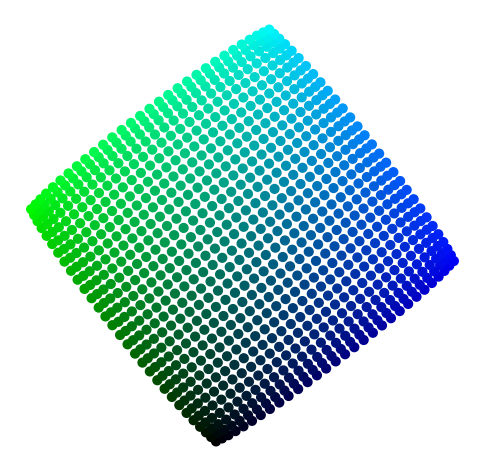
\includegraphics[width=5cm]{Task-1-t-SNE.png}
\end{figure}

\newpage

\bibliographystyle{unsrt}
\bibliography{bib}

\end{document}